\documentclass[10pt,a4paper]{article}
\usepackage[utf8]{inputenc}
\usepackage{amsmath}
\usepackage{amsfonts}
\usepackage{amssymb}
\usepackage{graphicx}
\begin{document}

\section*{Korrelationsmesstechnik - Task 2}

\[ x = (2,3,-2,4,5,-11), y = (4,5,-11,2,3,4) \]
\[ xcorr(x, y) = (8,18,5,6,5,24,-65,-65,162,-35,-44)\]

\[ x = (1,1,1,1,1,1), y = (3,0,-3,0,-3,0) \]
\[ xcorr(x, y) = (0, -3, -3, -6, -6, -3, -3, 0, 0, 3, 3)\]

\[ x = (0, 2, 2, 0, 0, 0, 2, 2, 0) \]
\[ autocorr(x) = (0,0,4,8,4,0,0,8,16,8,0,0,4,8,4,0,0) \]

\[ x = (0, 2, 0, 2, 0, 0, 2, 0), y = (2, 0, 2, 0, 2, 0, 2, 0) \]
\[ xcorr(x, y) = (0,0,4,0,8,0,8,4,8,4,4,4,0,4,0) \]

\section*{Stichproben - Task 1}

\subsection*{Mittelwerte und Varianzen}

x Mittelwert: $5.1416666667$, x Standardabweichung: $3.084995457$.

y Mittelwert: $2.5708333333$, y Standardabweichung: $1.56036976$

\subsection*{Covariance Matrix}

\[
\begin{pmatrix}
9.5172 & 4.7977 \\
4.7977 & 2.4348 \\
\end{pmatrix}
\]
\pagebreak
\subsection*{Correlation Coefficient}

\[
corr(x,y) = 0.99667
\]

The correlation coefficient suggests high correlation of the values, approaching linearity. A simple plot visualizes this further (see figure 1 below).

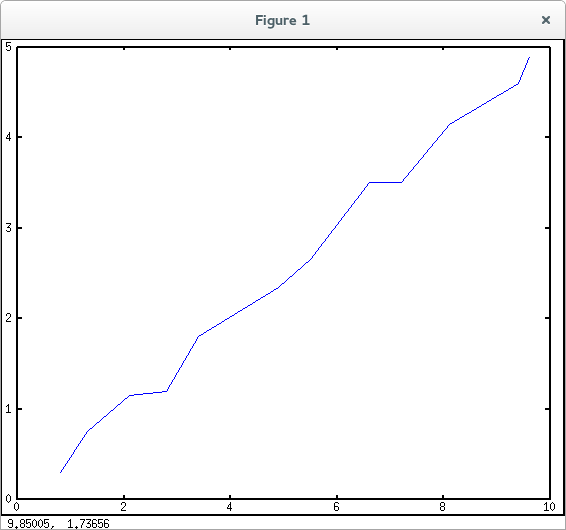
\includegraphics[scale=0.7]{fig1}

\pagebreak
\subsection*{Histograms}

After playing around a bit histograms with 4 bins seem to make most sense.

x histogram:

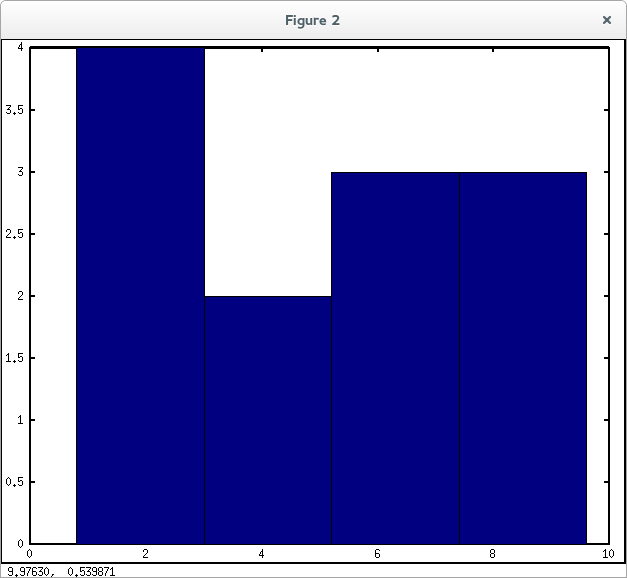
\includegraphics[scale=0.6]{xhist}

\pagebreak

y histogram:

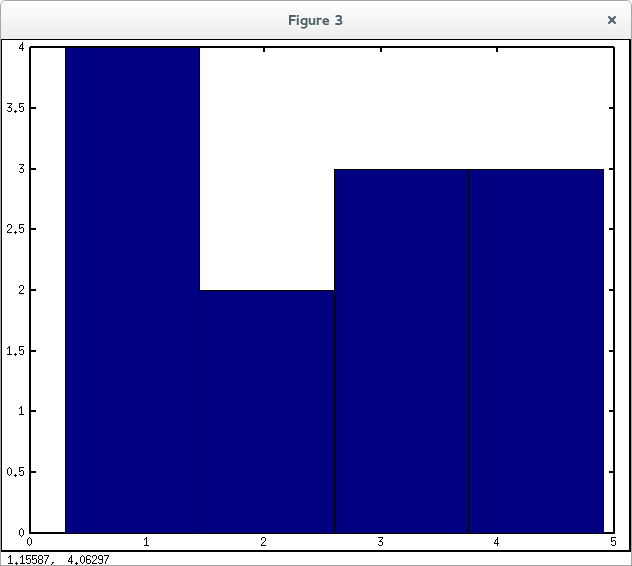
\includegraphics[scale=0.6]{yhist}

\end{document}